% !TEX root = ../main.tex

% Background section

\section{Background}

\subsection{Traditional Bootstrapping}
Bootstrapping is a relatively well-understood and widely used re-sampling method basically consisting of independent re-sampling steps with replacement. The paper by %~\cite{peskun}%
 \Peskun, however, makes us wonder if we can implement his idea of replacing independent re-sampling steps with dependent ones in the context of bootstrapping.

A typical bootstrapping process consists of the following:

\begin{enumerate}[label=\alph*)]
\item Given a set of samples S = $\{s_1, ..., s_n\}$, pick n samples with replacement from that set, generating a bootstrap sample $S^* = \{s^*_1, ..., s^*_n\}$.

\item Repeat this step m times.

\item Use your m bootstrap samples to estimate the distribution for a desired test statistic.
\end{enumerate}

We show a code in R as example, with a histogram in the following page:


\begin{lstlisting}

set.seed(547)
# number of iid random variables in our model
N = 500
# number of times the algorithm will run 
M = 1000 

# this distribution is unknown to the bootstrap user
x = rnorm(N, 2, 1.5)

bmeans = c()
bvars = c()

for (i in 0:M) {
  # randomly select N samples *with replacement* 
  bsample = sample(x, size=N, replace=TRUE) 
  
  bmean = mean(bsample)
  bmeans = c(bmeans, bmean)
  
  # example calculating another statistic: variance
  bvar = (N-1)/N*var(bsample)
  bvars = c(bvars, bvar)
  }

# plot histogram for means
hist(bmeans, breaks = 20)
\end{lstlisting}

\newpage

\begin{figure}
  \centering
	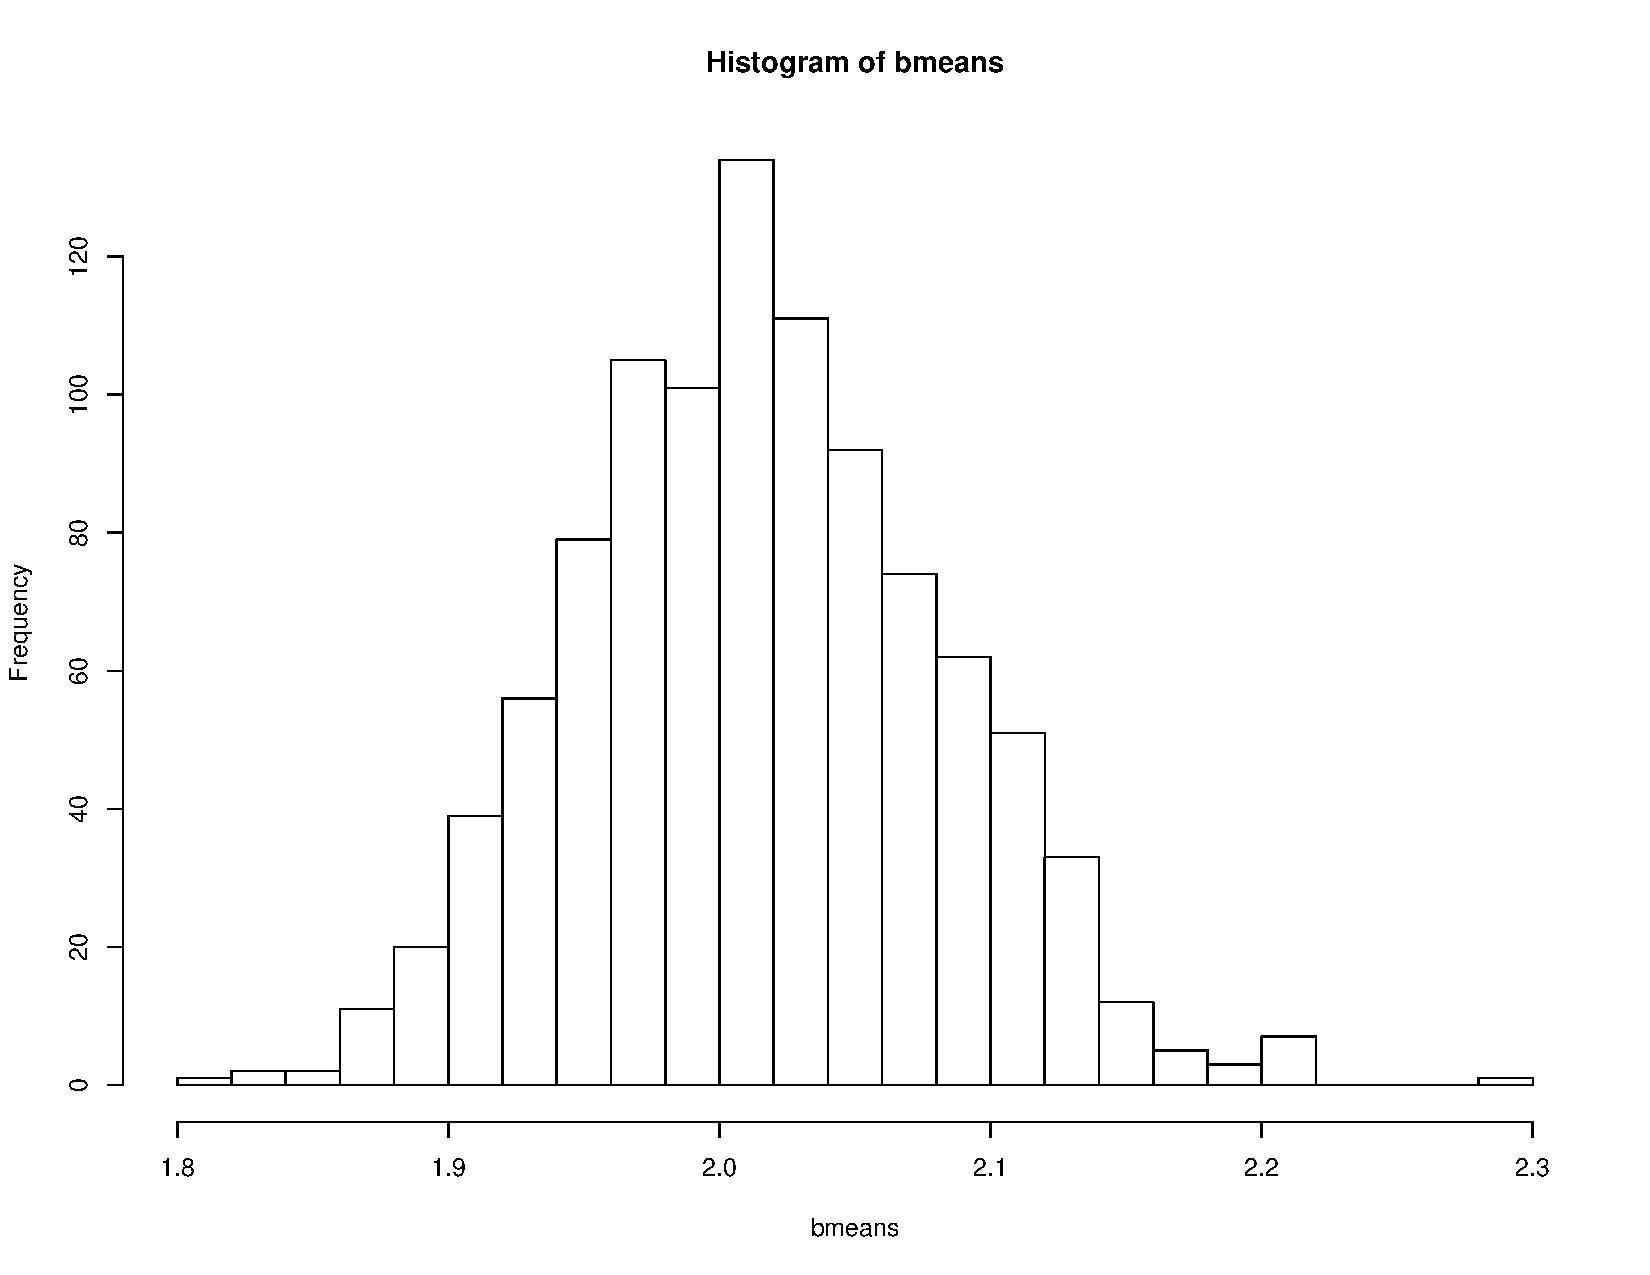
\includegraphics[scale=0.5]{hist_means.pdf}
	  \caption{A histogram of bootstrap means.}
\end{figure}




\subsection{Markov Chains}

The following the definitions and properties will be the base to the the second part of this project. The definitions and theorems in this section use as guide professors Ben's and Gyer's notes. I chose to add them here, even if not in depth, because they provide notions or vocabulary necessary to understand part 2.

\subsubsection{Transition Kernel}\label{kernel_section}

Transition Kernel definition: Let (E,$\calE$) and (F,$\calF$) be two measurable spaces, and let K be a mapping from E x $\calF$ into $\bar{R}_+$. Then K is called a\textbf{ transition kernel} from (E,$\calE$) into (F,$\calF$) if:

\begin{enumerate}[label=\alph*)]
\item for any fixed B in $\calF$, K(x,B), as a function of x, is E-measurable; and

\item\label{prob_meas} the mapping B $\rightarrow$ K(x,B) is a measure on (F,$\calF$) for every x in E.
\end{enumerate}

\subsubsection{Algebra of Kernels}\label{alg_kernels}
Given a measure $\lambda$, a measurable function f and kernels K, L, we have:

\begin{enumerate}[label=\alph*)]
\item$ \lambda K (B)  \overset{def}{=} \int \lambda(dx)K(x, B), B \in \calE.$ This operation will produce the \textbf{new measure} $\lambda K$.

\item$KL(x, B) \overset{def}{=} \int K(x, dy)L(y, B), B \in \calE.$. This operation will produce the \textbf{new kernel} $KL$. Notice that, by definition, $KL \neq LK$.
 
\item$Kf \overset{def}{=} \int K(x, dy)f(y)$ given that the integral exists. This operation will produce the \textbf{new measurable function} $Kf$. 

\end{enumerate}

\subsubsection{Definition: Markov Chain}

Special attention is given to \textbf{finite state spaces} in this section as they are the type of state space in our application.

A stochastic process $X_1, X_2, ...$ taking values in a measurable space, which is called the \textbf{state space}, is a \textbf{Markov chain} if the conditional distribution of the future given the past and present depends only on the present.

\textbf{Notation:} We assume the conditional distribution of $X_{n+1}$ given $X_n$ is given by a \textbf{Markov kernel P}, which is just a kernel that has a few extra properties. We will discuss more about it in the second part of the project.

\subsubsection{Finite state space: operations}
In section \ref{alg_kernels}, we defined operations in a familiar way, for instance being careful with the side by which we performed products, the same way we do when multiplying matrices. If we treat measurable functions as column vectors, kernels as matrices, and (probability) measures as row vectors, the operations work the same as the way we learned in a linear algebra course.

\subsubsection{Definition: Irreducible kernel}
A kernel P is irreducible if there is a measure $\varphi$ such that: for every $x \in E$ and $\varphi$-positive $A \in \calA$, there exists a positive integer n such that $P^n(x,A) > 0$. In such a case, we also say $\varphi$ is an irreducibility measure for P or P is $\varphi$-irreducible.

\subsubsection{Communicating states}
A set $B \in \calA$ is $\varphi$-communicating if for every $x \in B$ and every $\varphi$-positive $A \in A$ such that $A \subset B$ there exists a positive integer n such that $P_n(x,A) > 0$. A kernel P is $\varphi$-irreducible if and only if the whole state space is $\varphi$-communicating.

\subsubsection{Finite state space: irreducibility}
When we have a countable state space, irreducibility and existence of paths are associated.This will be the case in this project as our spaces will be more than countable: they will be finite. A \textbf{path} from $x = x_1$ to $y = x_n$ is a finite sequence of states $x_1, ..., x_n$ such that:
$ P (x_i, x_{i+1}) > 0, i = 1, ... , n - 1$.
If there exists a state y such that there is a path from x to y for every $x \in E$, then the kernel is irreducible.

\subsubsection{Theorem: Irreducible kernels and invariant measures}
A measure $\lambda$ is invariant (by a kernel K) if $\lambda K = \lambda$. If a Markov kernel is irreducible and has an invariant measure, then the invariant measure is unique up to multiplication by positive constants. A proof can be seen in Theorems 10.0.1 and 10.1.2 in Meyn and Tweedie (2009), which can be found in Gyer's notes.

%\subsubsection{Definition of Stationary Transition Probability}
%A Markov chain has stationary transition probabilities if the conditional distribution of $X_{n+1}$ given $X_n$ does not depend on n.

%%%%% new section %%%%%
\subsection{Estimation and variation}
In this section we will discuss a little notation and terminology used in estimation.

Assume we have an irreducible, Markov chain with discrete and finite states 1, ..., S. Recall that irreducibility guarantees that if there's an invariant measure $\pi$ for our kernel P, then that invariant measure is unique. Let f be a measurable function. Define A as:

\[
A = E_{\pi}[f(X)] =  \sum_{i=1}^S f(i) \pi
\]

We simulate our Markov chain with kernel P for times 1, ..., N and estimate A as follows:

\[
\tilde{A} = \sum_{t=1}^N f(X(t)) / N
\]

Let now the asymptotic variance $v(f, \pi, P)$ be

\[
v(f, \pi, P) = \lim_{N \rightarrow \infty } N \text{Var}(\tilde{A})
\]

Those quantities will be important when we discuss our research question.